% =========================================================
\section{TEF-RAG 方法}
\label{sec:method}
% =========================================================

图~\ref{fig:tef_overview} 给出 TEF-RAG 的整体流程。方法由四个相互衔接的阶段组成：合法候选检索、学习式证据对提议、查询条件化关系建图，以及非线性集合排序。前两步控制候选规模，关系图负责表示证据之间的过程结构，最终排序器直接选择最有用的证据集合。

\begin{figure*}[t]
    \centering
    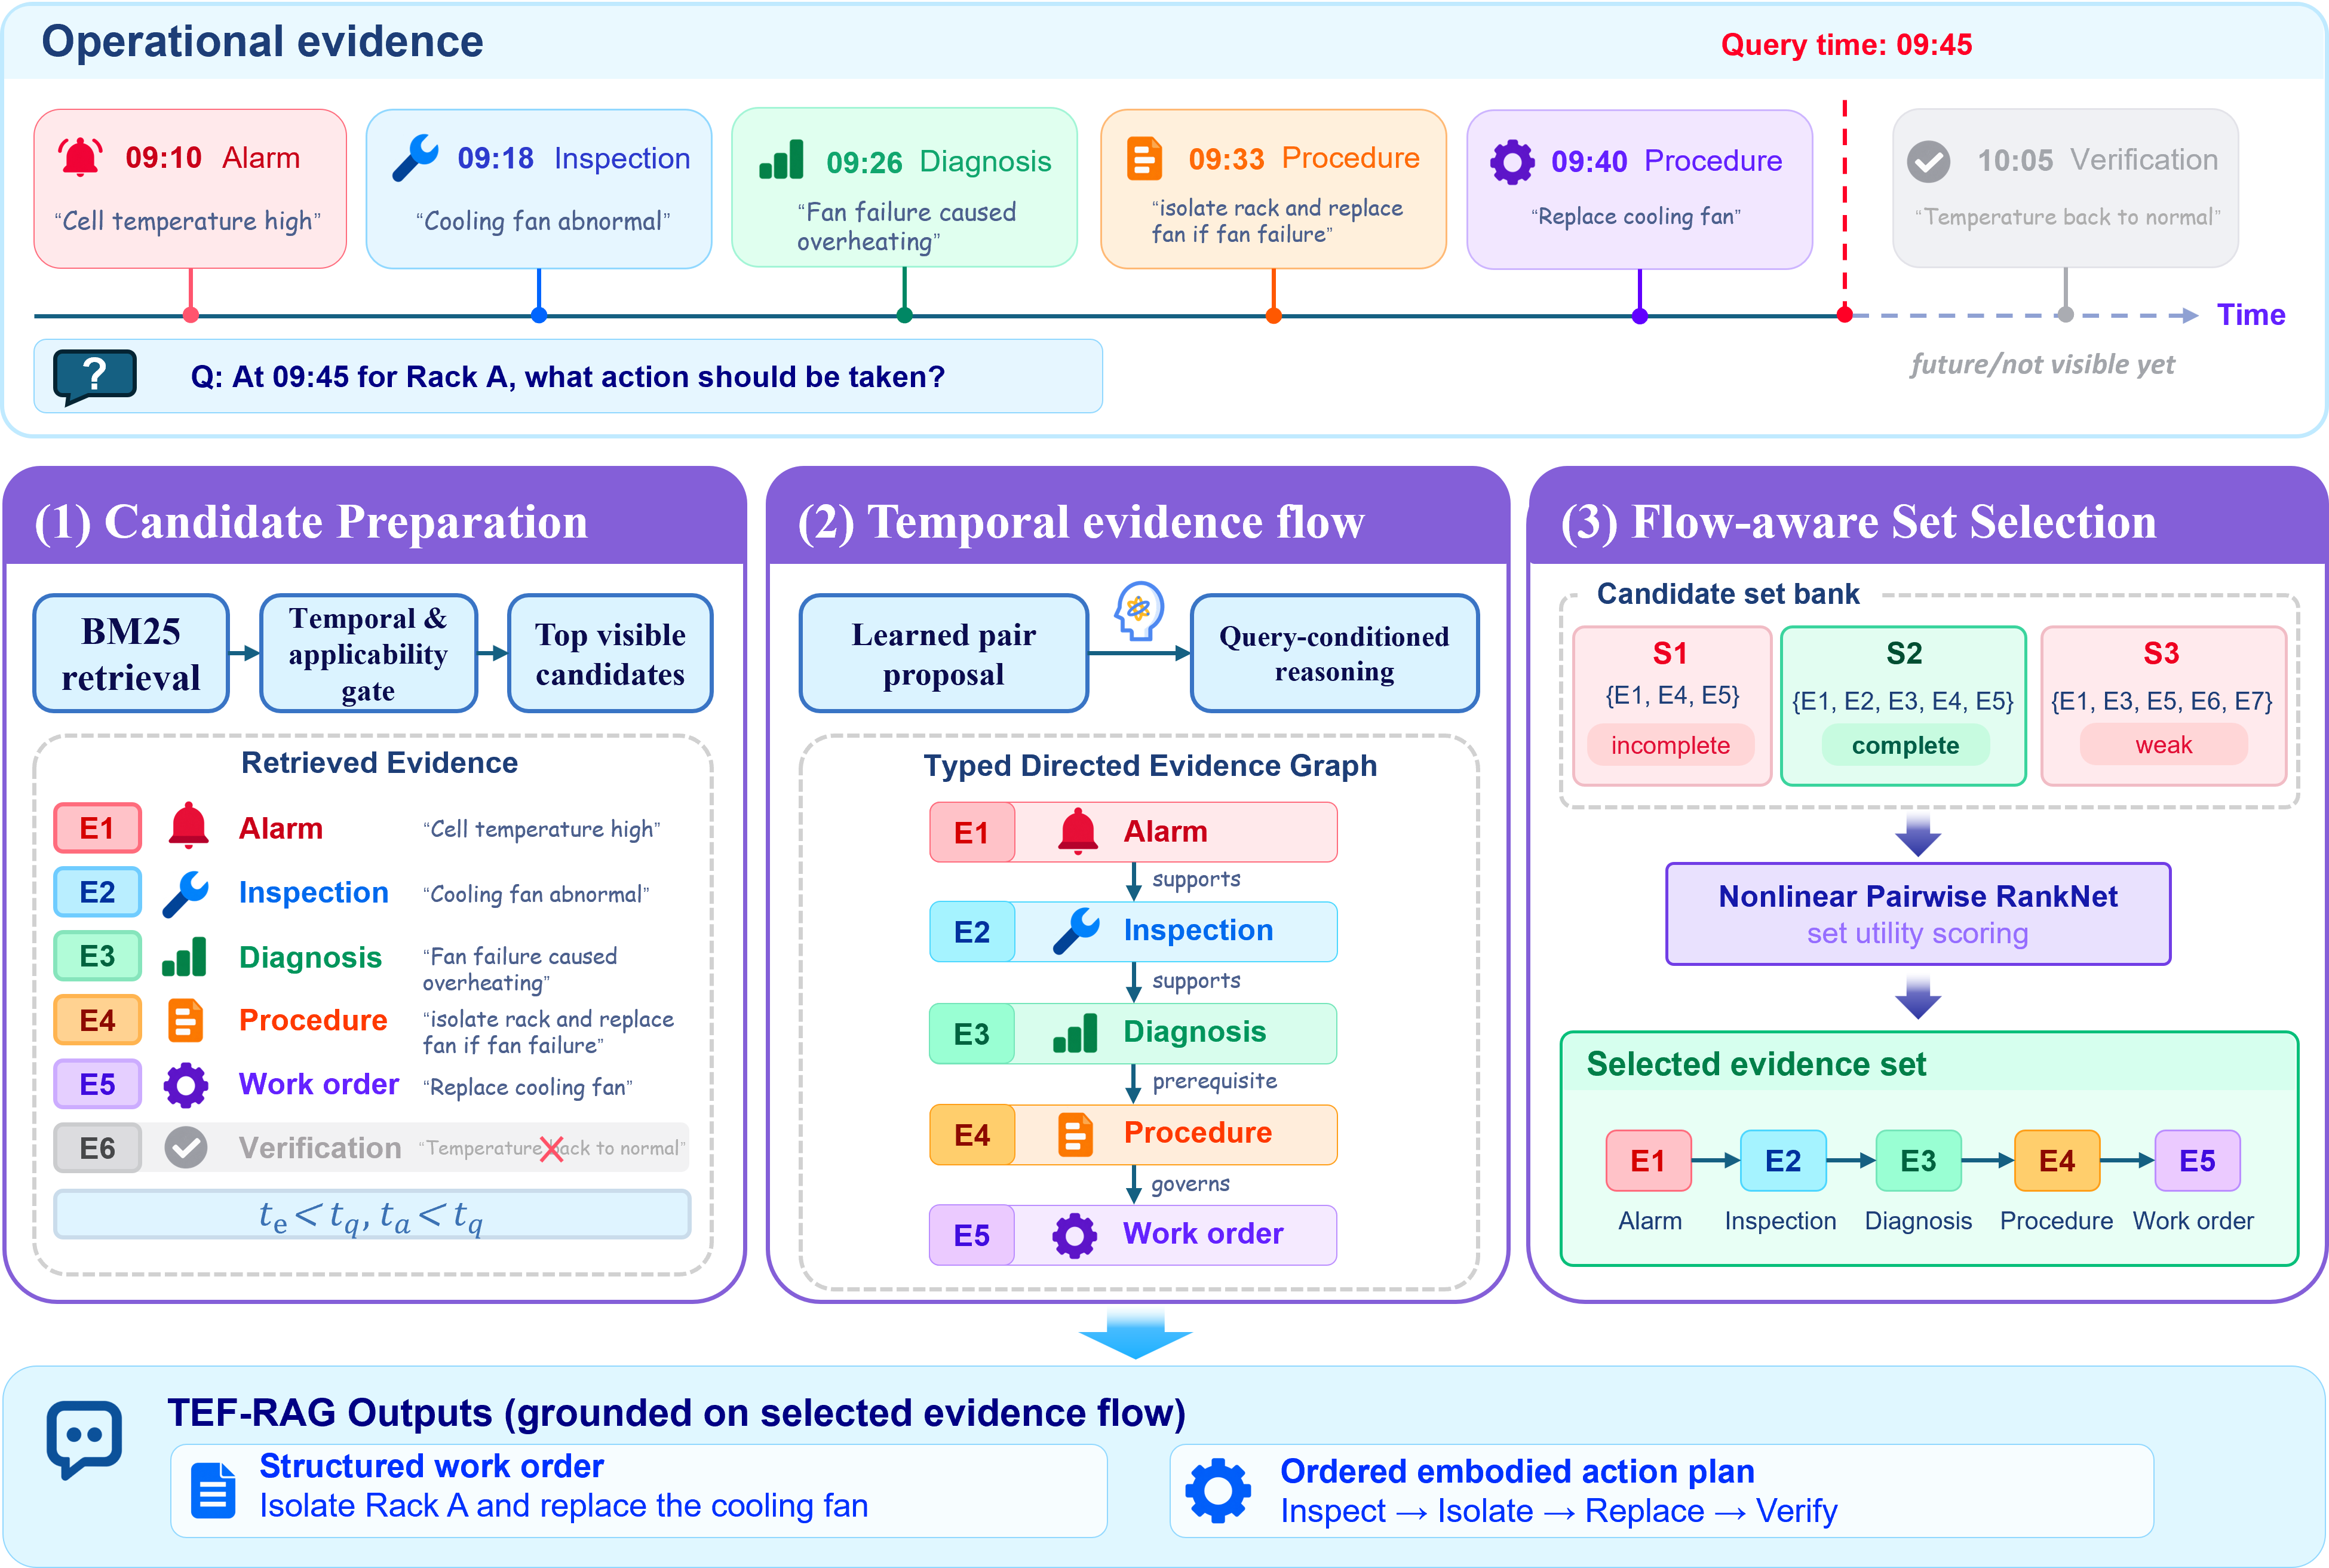
\includegraphics[width=0.96\textwidth]{figures/tef_rag_overview.png}
    \caption{TEF-RAG 总体框架。系统先在查询时刻合法的候选证据上筛选关系候选对，随后构建查询条件化的 Temporal Evidence Flow，并在候选集合空间中利用非线性 pairwise ranking 选择 Top-5 evidence flow；选出的证据作为统一下游生成器的受控上下文。}
    \label{fig:tef_overview}
\end{figure*}

\subsection{候选证据准备与时序合法性}

TEF-RAG 首先对原始异构记录执行统一的合法性检查。资产不一致、事件发生在查询之后、记录在查询之后才可用，以及不适用于当前型号或时段的规程都会被直接排除。这一步不学习“相关性”，而是建立不可被后续模型突破的知识边界。

在合法集合 $\Candidates_q$ 上，基础检索器产生较大的搜索池。其作用是保证召回率，而不是直接决定最终 Top-5。每个候选节点保留词法相关性、时间新近性、查询角色兼容性等部署时可计算的节点特征，供后续 pair proposal 与集合排序使用。

\subsection{学习式 Pair Proposal}

若对搜索池中全部有序证据对进行语义关系判断，成本会随候选数平方增长。TEF-RAG 因此先学习一个轻量 pair proposer，对每个时间顺序合法的证据对 $(e_i,e_j)$ 估计其“值得进入关系判断”的概率：
\begin{equation}
p_{ij}
=
\sigma\!\left(
\mathbf{w}^{\top}\phi_p(q,e_i,e_j)+b
\right).
\label{eq:pair_proposal}
\end{equation}

$\phi_p$ 只使用部署时可见特征，包括 query--source/target 与 source--target 词汇重合、两端节点分数、事件与来源类型、时间间隔、查询角色需求，以及显式 supersession 等元数据。随后按 $p_{ij}$ 排序，仅保留固定预算内的候选对。该模块只回答“哪些 pair 值得进一步判断”，并不预测最终关系类型。

这一设计有两个作用：一是把语义关系推理集中在更有希望的证据对上；二是学习传统规则难以覆盖的跨来源互补关系，同时保留时间方向这一确定性约束。

\subsection{查询条件化的 Temporal Evidence Flow}

对保留的候选对，关系判断模块在查询语境下预测是否存在语义边及其关系类型。最终图记为
\begin{equation}
\FlowGraph_q=(V_q,E_q),
\qquad
E_q\subseteq V_q\times\Rels\times V_q.
\end{equation}

关系词汇表覆盖 supports、governs、qualifies、contrasts、prerequisite、preserves uncertainty、resolves、supersession、updates 与 verifies 等过程关系。边方向遵循事件时间或明确的前置/更新方向，因此图可以形成分支和汇合，而不强制退化为单一路径。

与静态知识图不同，$\FlowGraph_q$ 是查询条件化的：同一条记录在不同查询下可能具有不同的重要性，不同证据对也可能因为当前任务角色不同而产生不同的有效关系。TEF-RAG 因而把“关系”视为当前检索问题的一部分，而不是语料预处理阶段固定不变的背景结构。

\subsection{候选证据集合构造}

关系图建立后，系统构造固定大小的候选集合库 $\SetBank_q$。候选集合来自高分节点的组合、已有贪心解以及其局部替换邻域。这里的目标不是穷举全部 $\binom{|V_q|}{5}$ 个组合，而是在可控规模内保留足够多的高质量、结构差异明显的候选。

对每个集合 $\Selected$ 提取集合级特征 $\phi_s(q,\Selected,\FlowGraph_q)$。这些特征包括：
\begin{itemize}
    \item 节点相关性、时间分数和角色兼容性的统计量；
    \item 事件类型与来源类型的覆盖度；
    \item 集合内部有效边数量、置信度、连通分量和最长有向路径；
    \item 时间跨度、平均事件间隔以及来源/文本多样性；
    \item 冗余、缺失角色与孤立节点等惩罚信号。
\end{itemize}

这些特征共同描述“这五条证据作为一个整体是否像一条完整证据流”，而不是简单重复单节点得分。

\subsection{非线性 Pairwise Set Ranking}

最终排序器采用小型非线性 RankNet。令
\begin{equation}
s_{\theta}(q,\Selected)
=
\operatorname{MLP}_{\theta}
\!\left(
\phi_s(q,\Selected,\FlowGraph_q)
\right),
\end{equation}
其中 MLP 为 $62\!\rightarrow\!64\!\rightarrow\!32\!\rightarrow\!1$ 的前馈网络。训练时不独立分类每个集合，而是在同一查询内构造成对偏好 $(\Selected^+,\Selected^-)$，并最小化
\begin{equation}
\mathcal{L}
=
-\log \sigma\!\left(
s_{\theta}(q,\Selected^+)
-
s_{\theta}(q,\Selected^-)
\right).
\label{eq:ranknet_loss}
\end{equation}

正集合满足离线定义的完整 evidence flow；负集合来自高启发式分数但不完整的候选。第一轮训练后，模型重新打分整个候选库，并把排名靠前的错误集合加入困难负样本，再进行第二轮训练。这样的 query-level hard-negative mining 使模型集中学习最容易混淆的“看起来相关但流程不完整”的集合。

推理时只计算候选集合的 $s_{\theta}$，选择得分最高的 Top-5 集合作为 $\hat{\Selected}_q$。至此，TEF-RAG 完成从节点召回、关系建图到集合级选择的全过程。

\subsection{与下游生成器的接口}

为隔离检索质量的影响，所有比较方法共享同一个下游生成器。生成器只接收查询与当前方法选出的证据记录，不接收方法名称、检索分数或 TEF 图结构。这样，生成结果的差异主要反映上游检索上下文的差异，而不是不同生成策略带来的混杂。
